\documentclass[12pt, a4paper]{article}
\usepackage[utf8]{inputenc}
\usepackage{amsmath}
\usepackage{relsize}
\usepackage{array}
\usepackage{xcolor}
\usepackage{courier}
\usepackage{listings}
\lstset{basicstyle=\footnotesize\ttfamily,breaklines=true}
\lstset{framextopmargin=50pt,frame=bottomline}
\usepackage{tikz}
\usetikzlibrary{calc}
\usepackage{graphicx}
\graphicspath{ {./images/} }
\usepackage{multirow}

\title{CSI3120 Assignment 4}
\author{Jake Wang}
\date{\today}

\begin{document}
	\maketitle
	
	\section*{Question 1}
	\begin{align*}
		\underline{(\lambda f.\lambda x.f\ x)(\lambda g.\lambda y.g\ y)}(\lambda z.z + 2)\ 3
		&= (\lambda x.\underline{(\lambda g.\lambda y.g\ y)\ x}) (\lambda z.z + 2)\ 3 \\
		&= \underline{(\lambda x.\lambda y.x\ y)(\lambda z.z + 2)}\ 3 \\
		&= \lambda y.(\underline{\lambda z.(z + 2)\ y})\ 3 \\
		&= \underline{(\lambda y.y + 2)\ 3} \\
		&= 3 + 2 \\
		&= 5
	\end{align*}
	
	\section*{Question 2}
	$$
		[(z + y + 1) / x]((\lambda y.\lambda z.(y - z) + x)\ x\ 0)
	$$
	Renaming bound variables $z$ and $y$ in the expression:
	$$
		[(z + y + 1) / x]((\lambda u.\lambda v.(u - v) + x)\ x\ 0)
	$$
	Subtitute unbound variable $x$ with $(z + y + 1)$:
	$$
		((\lambda u.\lambda v.(u - v) + (z + y + 1))\ (z + y + 1)\ 0)
	$$
	
	\section*{Question 3}
	\subsection*{(a)}
	Since arguments are passed by value, $x$ and $y$ will not change.
	$x = 5$ and $y = 1$.
	\\\\
	In $g(5, 1)$:
	\begin{itemize}
		\item $i = 5, j = 1$
		\item $j := j + i + 2 = 5 + 1 + 2 = 8$
		\item $i := i * j = 5 * 8 = 40$
		\item Returning $i + j = 40 + 8 = 48$
	\end{itemize}
	Therefore, $z = 48$.\\
	\\
	In $g(1, 1)$:
	\begin{itemize}
		\item $i = j = 1$
		\item $j := j + i + 2 = 1 + 1 + 2 = 4$
		\item $i := i * j = 1 * 4 = 4$
		\item Returning $i + j = 4 + 4 = 8$
	\end{itemize}
	Therefore, $w = 8$.
	\\
	Printed numbers are $5, 1, 48, 8$.

	\subsection*{(b)}
	Since arguments are passed by reference, $x$ and $y$ will change by $g$.
	\\
	Initially, $x = 5$ and $y = 1$.
	\\\\
	In $g(x, y)$:
	\begin{itemize}
		\item $i = 5, j = 1$
		\item $j := j + i + 2 = 5 + 1 + 2 = 8$
		\item $i := i * j = 5 * 8 = 40$
		\item Returning $i + j = 40 + 8 = 48$
	\end{itemize}
	Therefore, $x = 40$, $y = 8$ and $z = 48$.\\
	\\\\
	In $g(y, y)$:
	\begin{itemize}
		\item $i = 8, j = 8$
		\item $j := j + i + 2 = 8 + 8 + 2 = 18$
		\item $i := i * j = 8 * 18 = 144$
		\item Returning $i + j = 144 + 18 = 162$
	\end{itemize}
	Therefore, $x = 144$, $y = 18$ and $w = 162$.
	\\
	Printed numbers are $144, 18, 48, 162$.
	
	\section*{Question 4}
	\subsection*{(a)}
	\begin{center}
		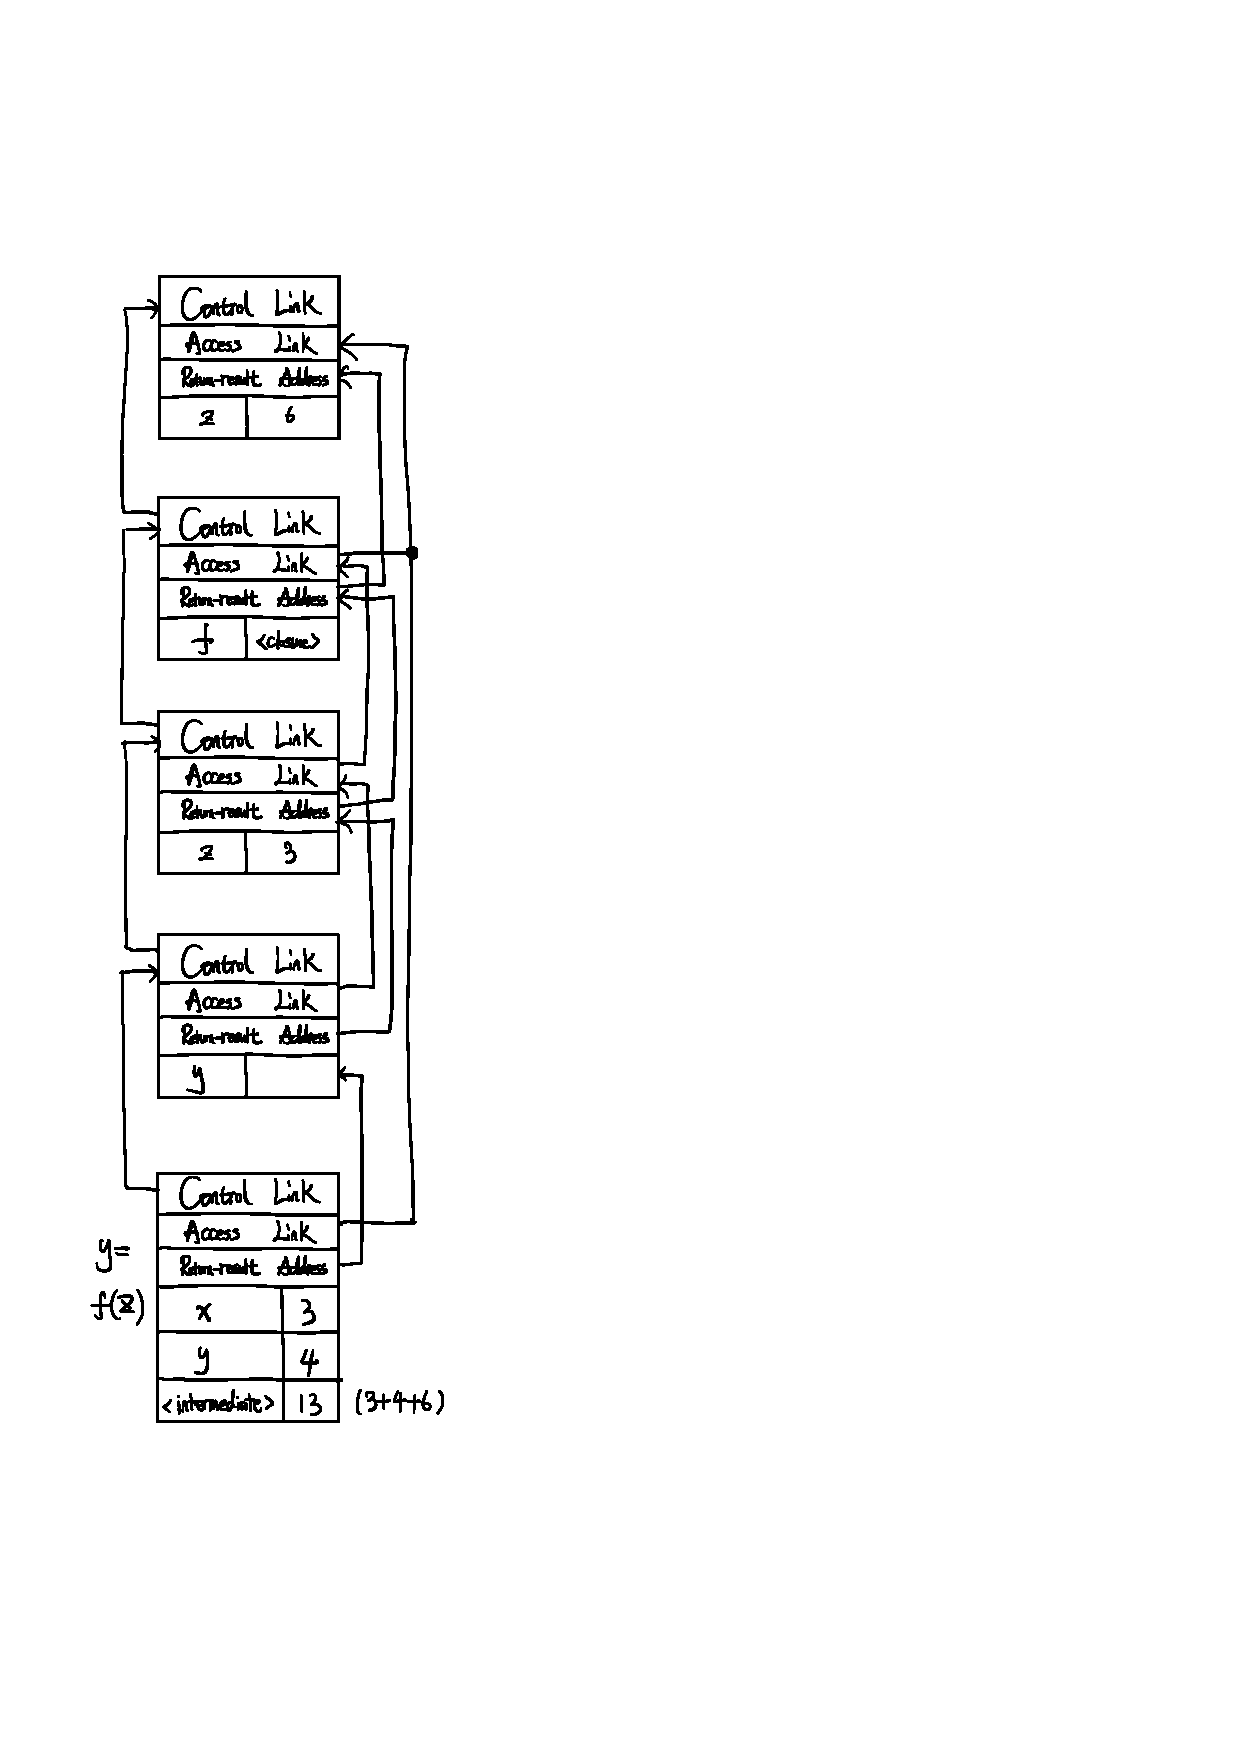
\includegraphics[scale=0.75]{Q4a.pdf}
	\end{center}
	
	\subsection*{(b)}
	The final value is 16. ($3 + 6 + 4 + 3$)
	
	\subsection*{(c)}
	\begin{center}
		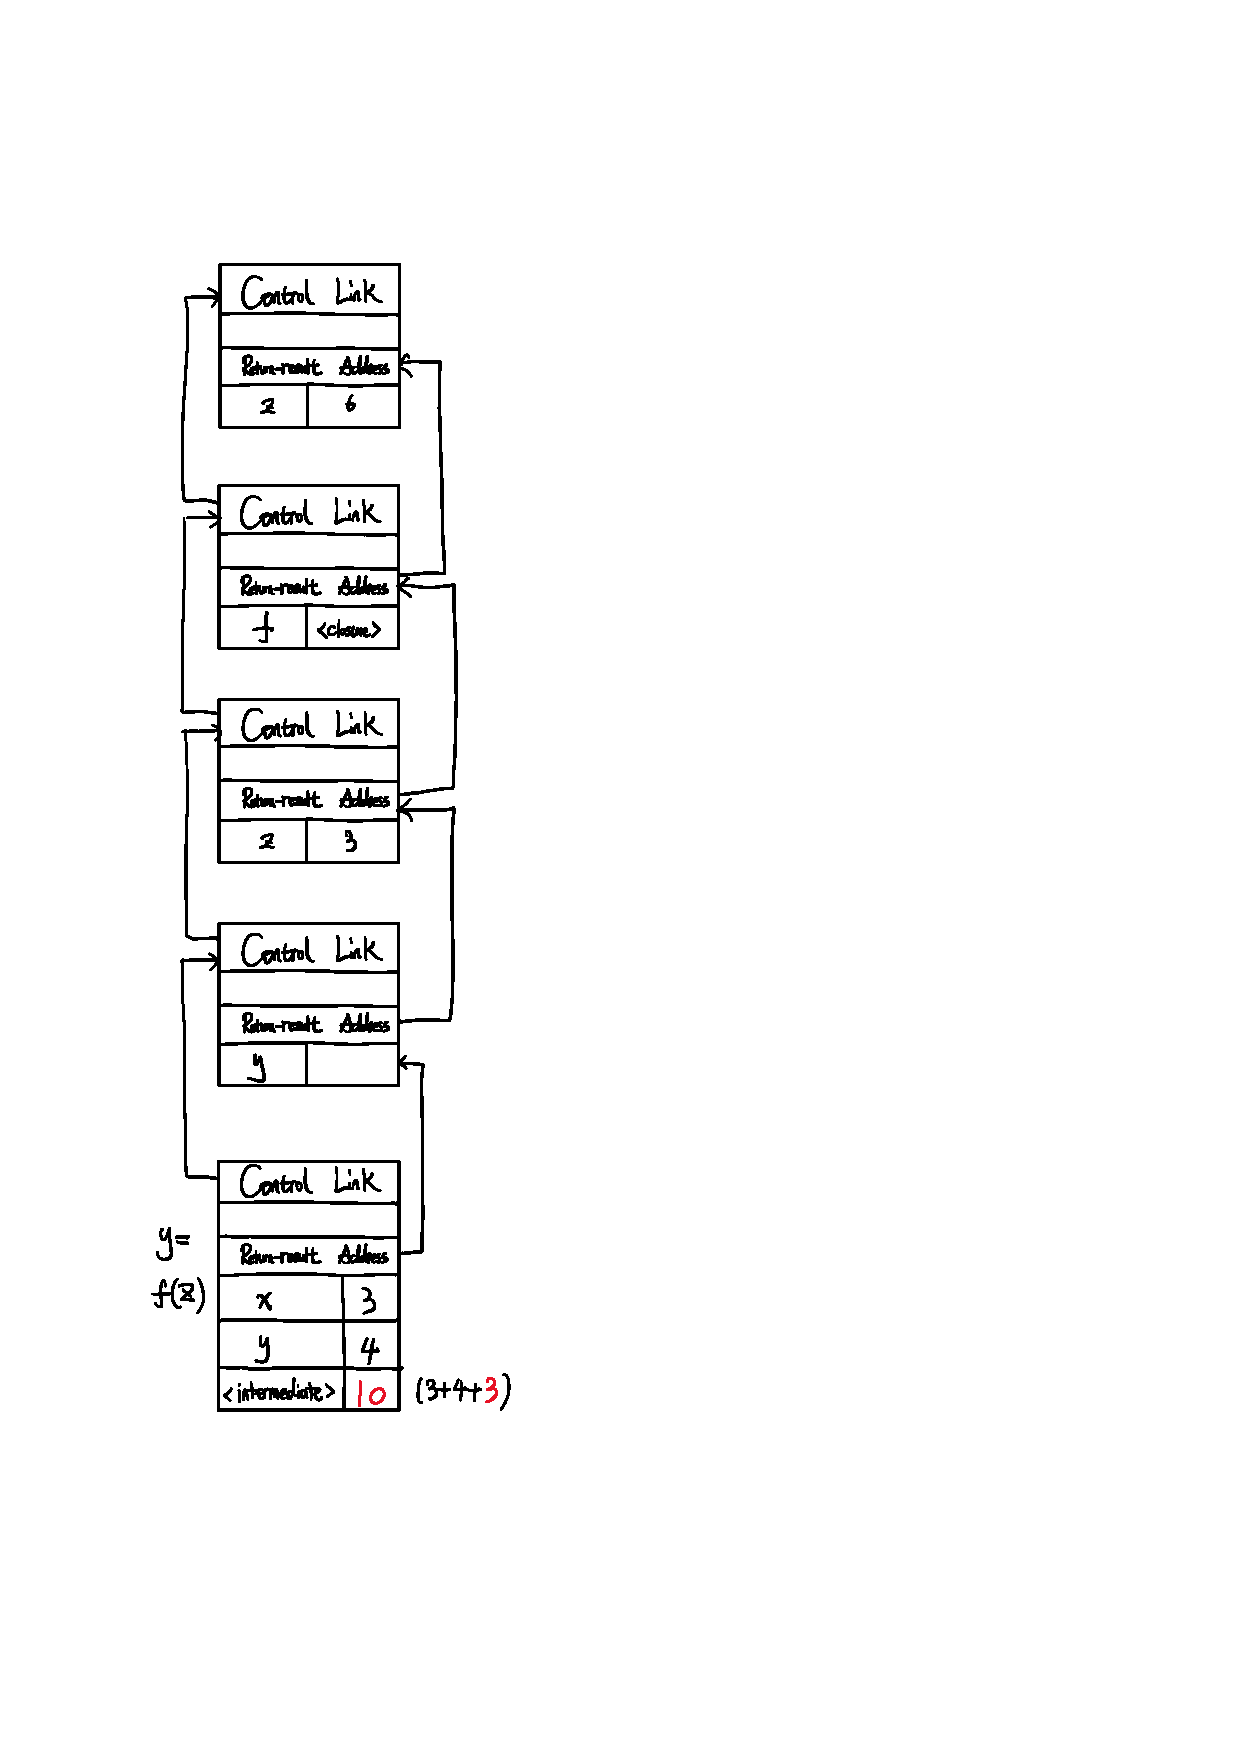
\includegraphics[scale=0.75]{Q4c.pdf}
	\end{center}
	
	
	\subsection*{(d)}
	The final value is 13. ($3 + 3 + 4 + 3$)
	
	\section*{Question 5}
	\begin{center}
		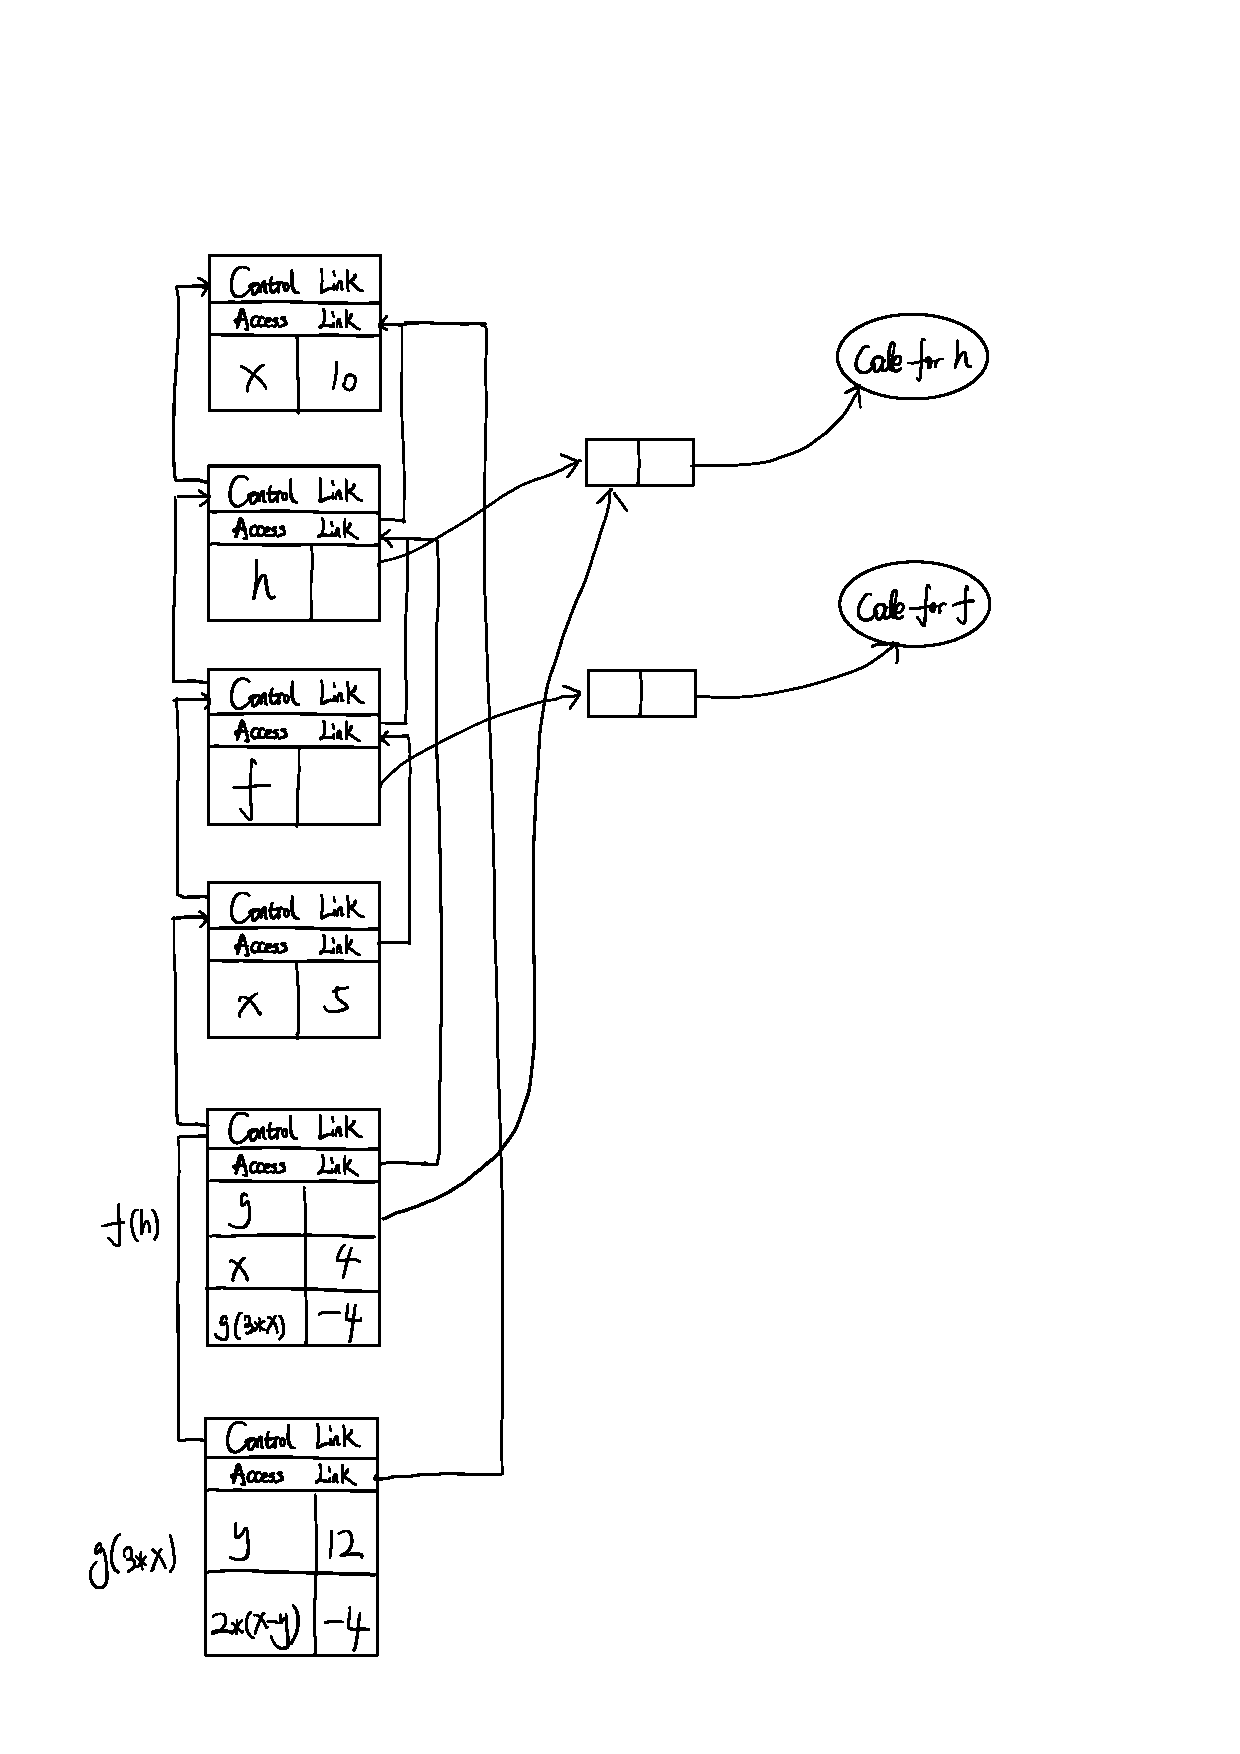
\includegraphics[scale=0.9]{Q5.pdf}
	\end{center}
	
\end{document}
